
% Asset ID: A21RadiansTikZ-002
% Purpose: Radian conversion circle for common angles.
\documentclass[tikz,border=8pt]{standalone}
\begin{document}
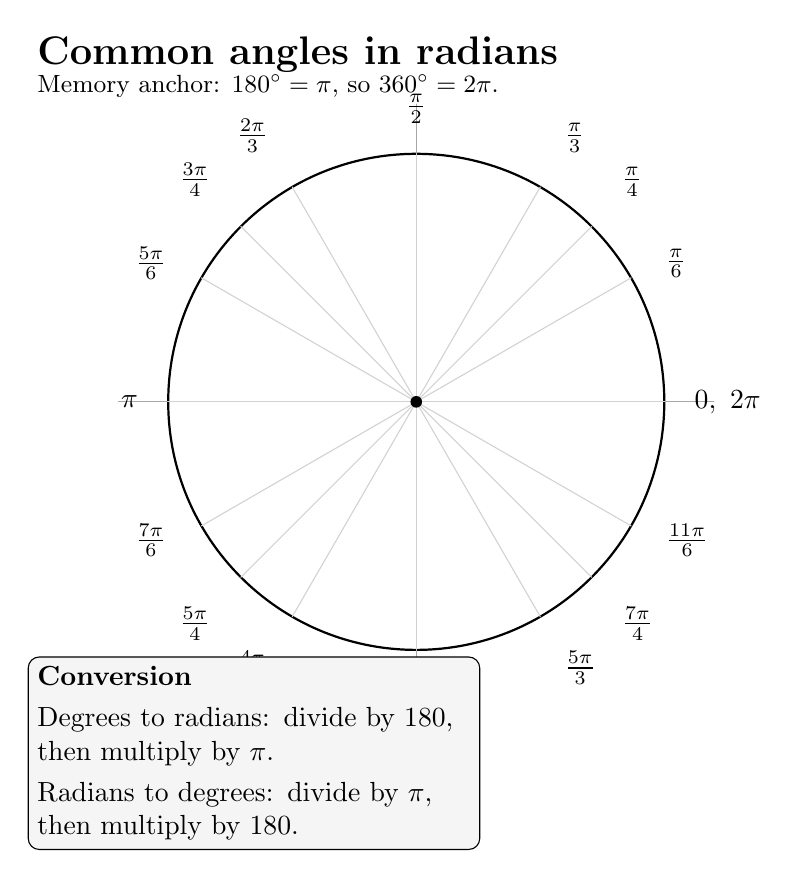
\begin{tikzpicture}[scale=1.05,line cap=round,line join=round]
\def\r{3}
\node[anchor=west,font=\bfseries\Large] at (-4.7,4.2) {Common angles in radians};
\node[anchor=west,font=\small] at (-4.7,3.82) {Memory anchor: \(180^\circ=\pi\), so \(360^\circ=2\pi\).};
\draw[thick] (0,0) circle (\r);\draw[gray!70] (-3.6,0)--(3.6,0);\draw[gray!70] (0,-3.6)--(0,3.6);
\foreach \a in {0,30,45,60,90,120,135,150,180,210,225,240,270,300,315,330}{\draw[gray!35] (0,0)--({\r*cos(\a)},{\r*sin(\a)});}
\node[right] at (3.25,0) {\(0,\ 2\pi\)};\node[above] at (0,3.25) {\(\frac{\pi}{2}\)};\node[left] at (-3.25,0) {\(\pi\)};\node[below] at (0,-3.25) {\(\frac{3\pi}{2}\)};
\node[right] at ({3.35*cos(30)},{3.35*sin(30)}) {\(\frac{\pi}{6}\)};\node[above right] at ({3.35*cos(45)},{3.35*sin(45)}) {\(\frac{\pi}{4}\)};\node[above right] at ({3.35*cos(60)},{3.35*sin(60)}) {\(\frac{\pi}{3}\)};
\node[above left] at ({3.35*cos(120)},{3.35*sin(120)}) {\(\frac{2\pi}{3}\)};\node[above left] at ({3.35*cos(135)},{3.35*sin(135)}) {\(\frac{3\pi}{4}\)};\node[left] at ({3.35*cos(150)},{3.35*sin(150)}) {\(\frac{5\pi}{6}\)};
\node[left] at ({3.35*cos(210)},{3.35*sin(210)}) {\(\frac{7\pi}{6}\)};\node[below left] at ({3.35*cos(225)},{3.35*sin(225)}) {\(\frac{5\pi}{4}\)};\node[below left] at ({3.35*cos(240)},{3.35*sin(240)}) {\(\frac{4\pi}{3}\)};
\node[below right] at ({3.35*cos(300)},{3.35*sin(300)}) {\(\frac{5\pi}{3}\)};\node[below right] at ({3.35*cos(315)},{3.35*sin(315)}) {\(\frac{7\pi}{4}\)};\node[right] at ({3.35*cos(330)},{3.35*sin(330)}) {\(\frac{11\pi}{6}\)};
\fill (0,0) circle (2pt);
\node[draw,rounded corners,fill=gray!8,align=left,anchor=west,text width=5.5cm] at (-4.7,-4.25) {\textbf{Conversion}\\[3pt]Degrees to radians: divide by \(180\), then multiply by \(\pi\).\\[3pt]Radians to degrees: divide by \(\pi\), then multiply by \(180\).};
\end{tikzpicture}
\end{document}
